% Spheres of squares from meanders (Section 3.2). Regions of the plane become vertices,
% pieces of river and road become edges, crossings become square faces.
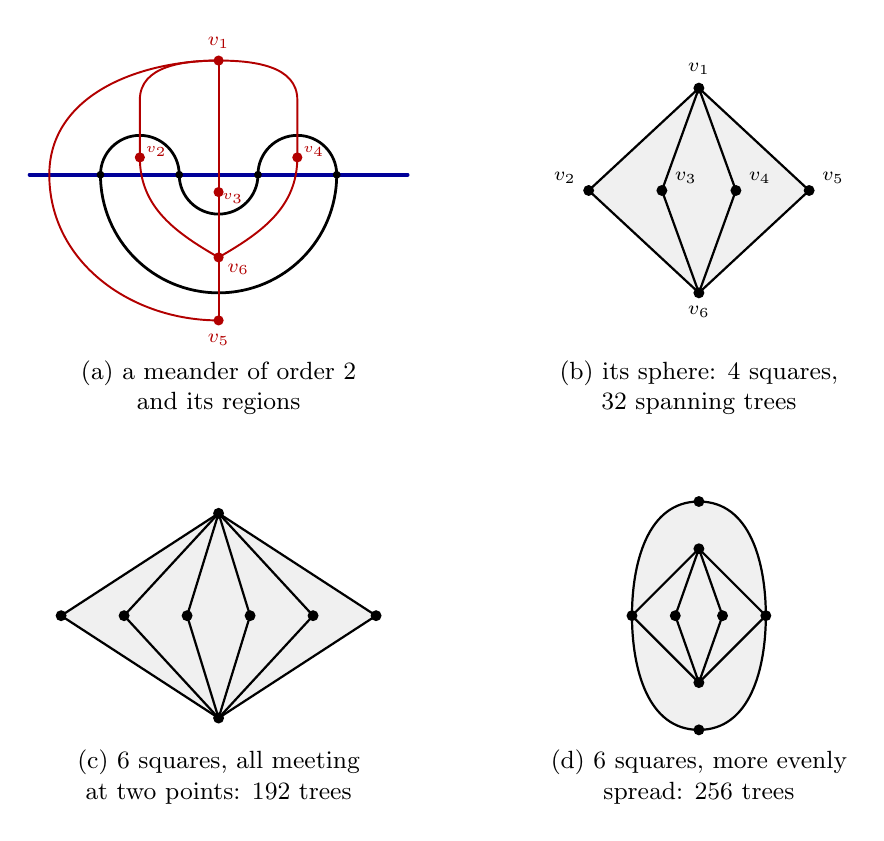
\begin{tikzpicture}[line cap=round]
  \tikzset{reg/.style={circle,fill=red!70!black,inner sep=1.3pt},
           dual/.style={red!70!black,line width=0.7pt},
           qv/.style={circle,fill=black,inner sep=1.4pt},
           qe/.style={line width=0.8pt},
           lab/.style={font=\scriptsize}}
  % ---------- (a) meander of order 2 with its regions ----------
  \begin{scope}[x=1cm,y=1cm]
    \draw[blue!60!black,line width=1.4pt] (0.1,0)--(4.9,0);
    \begin{scope}[line width=1pt]
      \draw (1,0) arc[start angle=180,end angle=0,radius=0.5];
      \draw (3,0) arc[start angle=180,end angle=0,radius=0.5];
      \draw (1,0) arc[start angle=180,end angle=360,radius=1.5];
      \draw (2,0) arc[start angle=180,end angle=360,radius=0.5];
    \end{scope}
    \foreach \k in {1,...,4} \fill (\k,0) circle[radius=1.4pt];
    % dual edges
    \draw[dual] (1.5,0.22)--(1.5,0.95) to[out=90,in=180] (2.5,1.45);
    \draw[dual] (3.5,0.22)--(3.5,0.95) to[out=90,in=0] (2.5,1.45);
    \draw[dual] (2.5,1.45)--(2.5,-0.22);
    \draw[dual] (1.5,0.22) to[out=-90,in=150] (2.5,-1.05);
    \draw[dual] (3.5,0.22) to[out=-90,in=30] (2.5,-1.05);
    \draw[dual] (2.5,-0.22)--(2.5,-1.05)--(2.5,-1.85);
    \draw[dual] (2.5,1.45) to[out=180,in=90] (0.35,0) to[out=-90,in=180] (2.5,-1.85);
    \foreach \p/\n/\a in {(1.5,0.22)/A/north,(3.5,0.22)/B/north,(2.5,1.45)/U/south,(2.5,-0.22)/C/east,(2.5,-1.05)/D/east,(2.5,-1.85)/L/north} {
      \node[reg] at \p {}; }
    \node[lab,font=\tiny,red!70!black] at (1.71,0.29) {$v_2$};
    \node[lab,font=\tiny,red!70!black] at (3.71,0.29) {$v_4$};
    \node[lab,red!70!black] at (2.5,1.68) {$v_1$};
    \node[lab,font=\tiny,red!70!black] at (2.68,-0.30) {$v_3$};
    \node[lab,red!70!black] at (2.75,-1.2) {$v_6$};
    \node[lab,red!70!black] at (2.5,-2.1) {$v_5$};
    \node[font=\small,align=center] at (2.5,-2.7) {(a) a meander of order $2$\\ and its regions};
  \end{scope}
  % ---------- (b) its sphere: four squares ----------
  \begin{scope}[xshift=8.6cm,yshift=-0.2cm]
    \fill[gray!12] (0,1.3)--(-1.4,0)--(0,-1.3)--(1.4,0)--cycle;
    \foreach \x/\n/\dx/\an in {-1.4/2/-0.04/east,-0.47/3/0.04/west,0.47/4/0.04/west,1.4/5/0.04/west} {
      \draw[qe] (0,1.3)--(\x,0)--(0,-1.3);
      \node[qv] at (\x,0) {}; \node[lab,anchor=\an] at (\x+\dx,0.16) {$v_\n$};}
    \node[qv] at (0,1.3) {}; \node[lab,anchor=south] at (0,1.35) {$v_1$};
    \node[qv] at (0,-1.3) {}; \node[lab,anchor=north] at (0,-1.35) {$v_6$};
    \node[font=\small,align=center] at (0,-2.5) {(b) its sphere: $4$ squares,\\ $32$ spanning trees};
  \end{scope}
  % ---------- (c) the six-square sphere where all squares meet at two points ----------
  \begin{scope}[yshift=-5.6cm,xshift=2.5cm]
    \fill[gray!12] (0,1.3)--(-2.0,0)--(0,-1.3)--(2.0,0)--cycle;
    \foreach \x in {-2.0,-1.2,-0.4,0.4,1.2,2.0} {
      \draw[qe] (0,1.3)--(\x,0)--(0,-1.3); \node[qv] at (\x,0) {};}
    \node[qv] at (0,1.3) {}; \node[qv] at (0,-1.3) {};
    \node[font=\small,align=center] at (0,-2.05) {(c) $6$ squares, all meeting\\ at two points: $192$ trees};
  \end{scope}
  % ---------- (d) the six-square sphere of the meander of Figure 1 ----------
  \begin{scope}[yshift=-5.6cm,xshift=8.6cm]
    \coordinate (U) at (0,0.85); \coordinate (C) at (0.85,0); \coordinate (G) at (0,-0.85); \coordinate (E) at (-0.85,0);
    \fill[gray!12] (C) to[out=90,in=0] (0,1.45) to[out=180,in=90] (E) to[out=-90,in=180] (0,-1.45) to[out=0,in=-90] (C);
    \draw[qe] (U)--(C)--(G)--(E)--cycle;
    \draw[qe] (U)--(-0.3,0)--(G);
    \draw[qe] (U)--(0.3,0)--(G);
    \draw[qe] (C) to[out=90,in=0] (0,1.45) to[out=180,in=90] (E);
    \draw[qe] (C) to[out=-90,in=0] (0,-1.45) to[out=180,in=-90] (E);
    \foreach \p in {(U),(C),(G),(E),(0,1.45),(0,-1.45),(-0.3,0),(0.3,0)} \node[qv] at \p {};
    \node[font=\small,align=center] at (0,-2.05) {(d) $6$ squares, more evenly\\ spread: $256$ trees};
  \end{scope}
\end{tikzpicture}
